\chapter{Literature Review}
\section{Existing Tools and Techniques}

\subsection{Imatest}
Imatest is a comprehensive software suite used for image quality testing developed by Imatest LLC\footnote[1]{https://www.imatest.com/}. It offers various modules to measure sharpness, noise, color accuracy, and other image quality factors using standardized test charts. Imatest's strengths lie in its extensive feature set and professional-grade accuracy. It is widely used in the industry by camera manufacturers, lens designers, and quality assurance teams. However, its complexity and cost can be prohibitive for amateur photographers.

Imatest employs a range of test charts and analytical techniques to evaluate lens performance. For example, it uses the SFRplus chart to measure spatial frequency response, which is crucial for assessing sharpness. The software also provides tools for analyzing distortion, chromatic aberration, and dynamic range. Despite its robustness, the steep learning curve and the need for specialized equipment make it less accessible to non-professional users \cite[]{ImatestAbout}.

\begin{figure}[h]
\centering
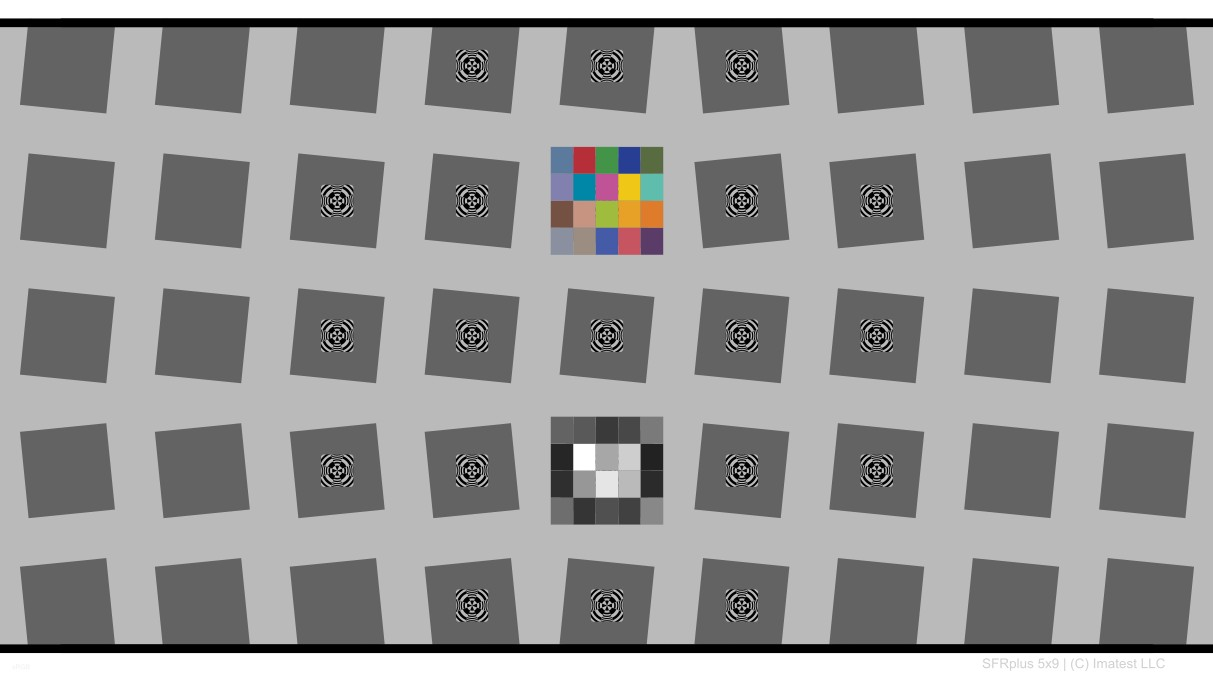
\includegraphics[height=5cm]{Images/SFRplus_chart.jpg}
\caption{Standard SFRplus test chart \cite{ImatestSFRChart}}
\label{fig:psf}
\end{figure}

\subsection{Dxomark}
Dxomark, a website by DXOMARK Image Labs\footnote[1]{https://www.dxomark.com/partners/}, provides image quality ratings for cameras, lenses, and mobile devices. Their tests include assessments of sharpness, exposure, color, noise, and optical distortions using standardized methodologies. Dxomark's ratings are industry-recognized and often cited by consumers and professionals alike when making purchasing decisions. The proprietary nature of its testing methods, however, limits user transparency and replicability \cite{DxomarkTestingLenses}.

Dxomark's lens testing protocol involves capturing images of various test scenes and charts under controlled conditions. They measure sharpness using a test chart with fine details and evaluate optical distortions by photographing grid patterns. Dxomark also assesses bokeh by analyzing images of defocused point light sources. While the results are comprehensive and reliable, the lack of detailed methodological disclosure means users cannot easily replicate the tests \cite{DxomarkBokeh}.

\subsection{Other Relevant Tools}
Beyond Imatest and Dxomark, several other tools and techniques are used for lens evaluation, including the Gletscherbruch Test and techniques measuring the sharpness and resolving power of an imaging system: the Edge Spread Function and the Line Spread Function.

\textbf{Gletscherbruch Test} evaluates decentering of a lens, which is a common issue where elements within the lens are not perfectly aligned, leading to blurriness and poor quality. The lens is first focused on a central target, then, without adjusting focus, the camera is moved to position the target in different corners of the frame. A decentered lens will show noticeable sharpness variations in different corners \cite{Gletscherbruch}.

The \textbf{Edge Spread Function} (ESF) describes how a sharp edge is reproduced. It measures the response of the imaging system to a high-contrast edge, capturing the transition from low to high intensity across the boundary of two areas. ESF is critical for analyzing how sharp or blurred an edge appears in an image \cite{ESF}.

The \textbf{Line Spread Function} (LSF) describes the response to a line. The LSF is derived from the ESF by taking its derivative, providing a one-dimensional representation of how a thin line would appear when imaged by the system \cite{ESF}.

\section{Key Concepts in Optical Image Quality Evaluation}

\subsection{Point Spread Function (PSF)}
The Point Spread Function (PSF) describes how a point source of light is imaged by an optical system. It represents the system's response to a point source and is a critical factor in determining image sharpness. A smaller PSF indicates better resolving power and sharper images \cite{PSFdescription}.

\begin{figure}[h]
\centering
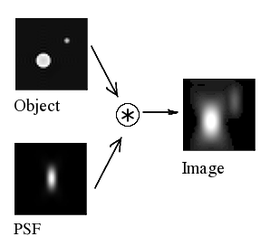
\includegraphics[width=3.7cm]{Images/psf.png}
\caption{Example of Point Spread Function \cite{PSF}}
\label{fig:psf}
\end{figure}

\subsection{Modulation Transfer Function (MTF)}
The Modulation Transfer Function (MTF) measures the ability of an optical system to reproduce (transfer) contrast from the subject to the image at various spatial frequencies. It is a crucial metric for assessing image sharpness. The MTF curve shows how contrast varies with spatial frequency, with higher values indicating better performance \cite{MTF}.

\begin{figure}[h]
\centering
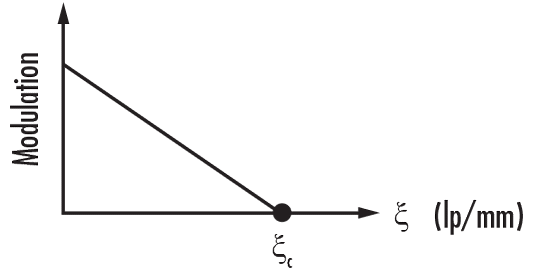
\includegraphics[height=3.5cm]{Images/MTF_example.png}
\caption{Example of Modulation Transfer Function for an Aberration-Free Lens with a Rectangular Aperture \cite{MTFimage}.}
\label{fig:mtf}
\end{figure}

\subsection{Optical Transfer Function (OTF)}
The Optical Transfer Function (OTF) combines the MTF and phase information to provide a complete description of the imaging system's performance. While the MTF only considers amplitude, the OTF includes both amplitude and phase, offering a more comprehensive view of how an optical system handles different spatial frequencies.

\begin{figure}[h]
\centering
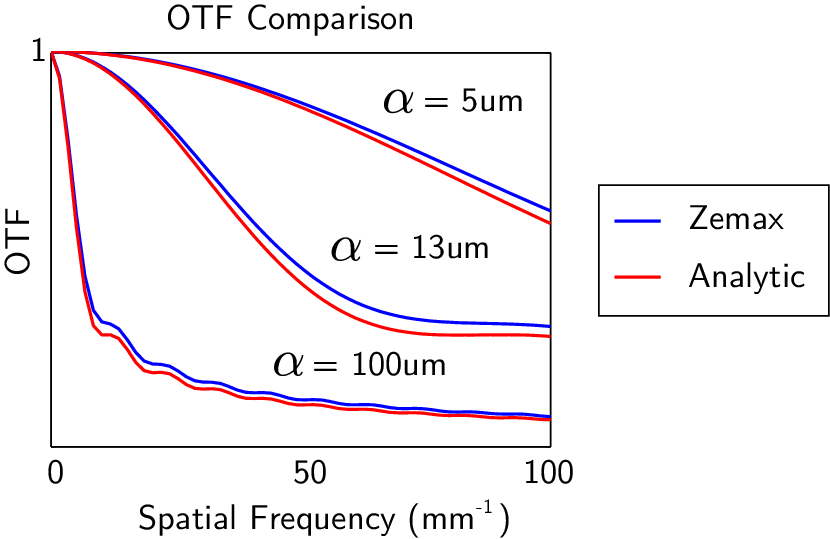
\includegraphics[height=5cm]{Images/OTF_example.png}
\caption{Example of Optical Transfer Function for a lens with spherical aberration \cite{OTFimage}}
\label{fig:otf}
\end{figure}

\section{Additional Concepts and Techniques}

\subsection{Image Quality Metrics}

\subsubsection{Accutance}
Accutance is a measure of perceived sharpness, taking into account both the contrast at edges and the human visual system's sensitivity to different spatial frequencies. It combines sharpness and contrast to provide a more comprehensive assessment of image quality \cite{accutance} .

\subsubsection{Sharpness and Optical Resolution}
Sharpness refers to the clarity and detail of an image, while resolution measures the amount of detail an imaging system can capture, typically in pixels. Higher resolution allows for larger prints and more detailed images.

\subsubsection{Dynamic Range}
Dynamic range is the range of light intensities a camera can capture, from the darkest shadows to the brightest highlights. High dynamic range (HDR) imaging techniques are used to enhance detail in both dark and bright areas.

\subsubsection{Noise}
Noise refers to random variations in pixel values, often visible as graininess or speckles in an image. It is more pronounced in low-light conditions and high ISO settings.

\subsubsection{Color Accuracy}
Color accuracy measures how faithfully a camera reproduces colors compared to the original scene. It is critical for applications requiring precise color reproduction, such as product photography and medical imaging.

\subsection{Lens-Induced Imperfections}

\subsubsection{Geometric Distortions}
Image distortions occur when straight lines in an image get unnaturally curved or deformed. Distortions are caused by aberrations near the edges of the image and can result from the use of certain lenses. Common types of distortion include barrel distortion, where lines bulge outward, typically seen when a lens is at full zoom; pincushion distortion, where lines curve inward, frequently associated with telephoto lenses; and waveform distortion, a combination of both barrel and pincushion distortions, often occurring with wide-angle cameras in zoom mode \cite{distortions}.

\begin{figure}[htbp]
  \centering
  \begin{subfigure}[b]{0.45\textwidth}
    \centering
    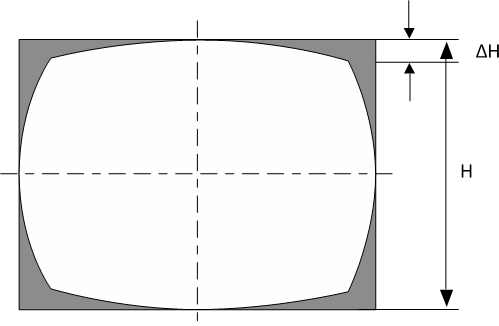
\includegraphics[height=3.3cm]{Images/barrel_distortion.png}
    \caption{Barrel distortion}
    \label{fig:barrel}
  \end{subfigure}
  \hfill
  \begin{subfigure}[b]{0.45\textwidth}
    \centering
    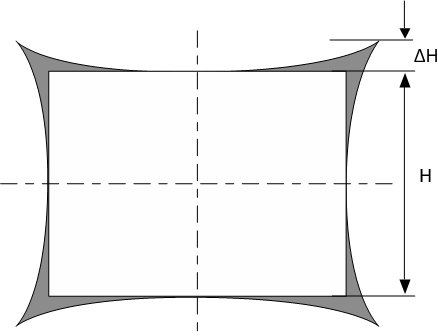
\includegraphics[height=3.3cm]{Images/pincushion_distortion.png}
    \caption{Pincushion distortion}
    \label{fig:pincushion}
  \end{subfigure}
  \caption{Examples of distortions \cite{distortions}.}
  \label{fig:distortions}
\end{figure}

\subsubsection{Chromatic Aberrations}
Chromatic aberration is an optical phenomenon caused by a lens failing to focus different wavelengths of light at the same point. There are two types of chromatic aberrations: longitudinal (axial), where different wavelengths of color do not converge at the same point after passing through a lens, and lateral, where different wavelengths of color coming at an angle focus at different positions along the same focal plane. Chromatic aberrations can degrade image quality and are typically corrected through lens design or software post-processing \cite{ChromaticAberation}.

\begin{figure}[h]
\centering
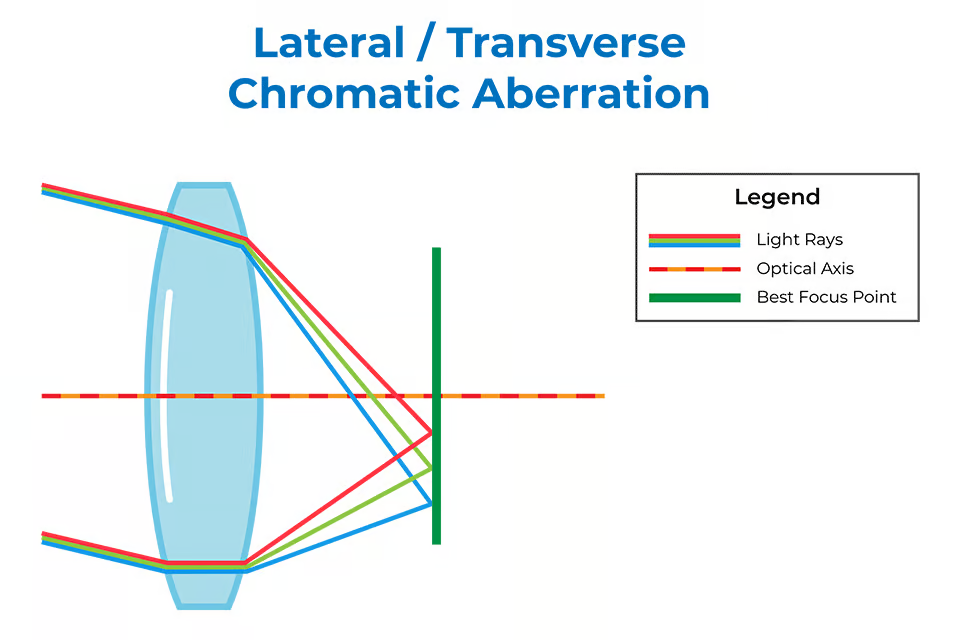
\includegraphics[height=4cm]{Images/chromatic_aberation.png}
\caption{Lens with lateral chromatic aberration \cite{ChromaticAberation}.}
\label{fig:chrom_ab}
\end{figure}

\begin{figure}[h]
\centering
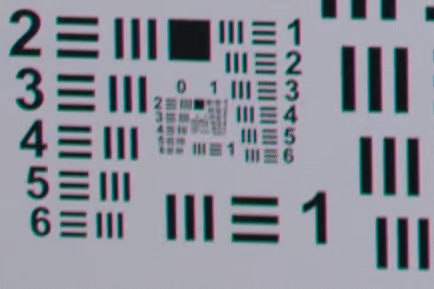
\includegraphics[height=2.9cm]{Images/chromatic_aberation_photo.png}
\caption{Example of a chromatic aberration \cite{ChromaticAberation}}
\label{fig:chrom_ab}
\end{figure}

\subsection{Aesthetic and Physical Lens Characteristics}

\subsubsection{Bokeh}
Bokeh describes the aesthetic quality of the out-of-focus areas in an image, often characterized by the shape and smoothness of background blur produced by the lens. Bokeh depends on lens aperture shape and size as well as other lens characteristics.

\subsubsection{Airy Disk}
An Airy disk is the diffraction pattern produced by a circular aperture, representing the fundamental limit of resolution for optical systems. It appears as a central bright spot surrounded by concentric rings of decreasing intensity. The diameter of the Airy disk depends on the wavelength of the light and the size of the aperture. \cite{AiryDisk}.

\begin{figure}[htbp]
\centering
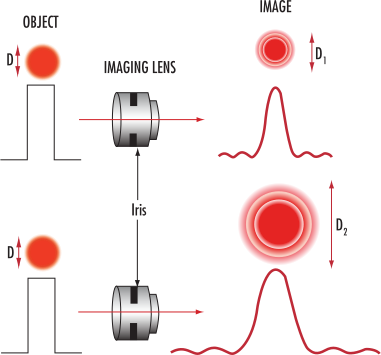
\includegraphics[height=5cm]{Images/airy_disk.png}
\caption{Airy disks depend on size of imaging lens aperture \cite{AiryDisk}}
\label{fig:airy_disk}
\end{figure}

\subsection{Digital Artifacts}

\subsubsection{Aliasing}
Aliasing occurs when a signal is undersampled, causing different signals to become indistinguishable. Aliasing is related to maximum spatial frequency, called the Nyquist frequency. Any information above the Nyquist frequency that reaches the sensor will be aliased to a lower spatial frequency and create visual artifacts. In imaging, it manifests as jagged edges or moiré patterns, especially when capturing fine details \cite{Aliasing}.

\begin{figure}[htbp]
\centering
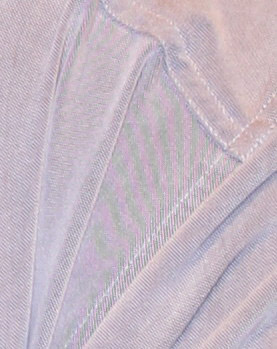
\includegraphics[height=5cm]{Images/color_moire.jpg}
\caption{Color Moiré pattern, an example of aliasing \cite{Aliasing}}
\label{fig:moire}
\end{figure}

\subsubsection{Focus Breathing}
Focus breathing refers to the change in a lens's field of view when adjusting focus, noticeable as a slight zooming effect during focusing \cite{FocusBreathing}.

\subsection{Testing and Calibration Tools}

\subsubsection{Test Charts}
Test charts are printed or digital patterns with known properties used to evaluate and calibrate the performance of imaging systems, assessing parameters like resolution, color accuracy, and distortion.

\section{Software Libraries and Tools}

\subsection{Camera Control Libraries}
\subsubsection{gphoto2}
The gphoto2 library provides a robust foundation for interfacing with digital cameras. It offers several key capabilities essential for lens testing including direct camera control through USB connections, remote capture capabilities, access to camera settings and configurations, support for multiple camera manufacturers, and RAW image capture support \cite{gphoto2}.

The library's architecture enables programmatic control of camera functions, making it possible to automate test sequences and ensure consistent capture conditions across multiple tests. The API provides both high-level functions for simple operations and low-level access for complex control requirements.

\subsection{Image Processing Libraries}
\subsubsection{OpenCV}
OpenCV (Open Source Computer Vision Library) serves as a cornerstone for lens analysis applications \cite{opencv}. Its capabilities include advanced edge detection algorithms crucial for MTF calculations, along with image filtering and noise reduction techniques. It also includes geometric distortion analysis, color space conversions, and efficient image manipulation routines to enhance the accuracy and efficiency of lens evaluation processes.

The library's optimized algorithms make it particularly suitable for real-time analysis of high-resolution images, a crucial requirement for lens testing applications.

\subsubsection{rawpy}
rawpy is a powerful library that offers essential capabilities for working with RAW image files. Its features include direct access to sensor data, debayering algorithms, color space conversion, exposure adjustment, and white balance control \cite{rawpy}.

These functionalities are critical for lens testing, as they allow access to unprocessed sensor data. This raw data provides a more accurate foundation for analyzing lens characteristics, ensuring precise and reliable results. By leveraging rawpy, the application enhances the overall quality of lens evaluation.

\subsection{Modern Web Frameworks}
\subsubsection{NiceGUI}
NiceGUI is a modern Python web framework designed to meet the needs of scientific applications, offering a range of features that enhance usability and performance \cite{nicegui}. It enables real-time updates without requiring page refreshes. The framework integrates seamlessly with Python-based data processing, allowing for efficient workflows in data-driven applications. Its modern reactive UI components provide an intuitive and interactive interface, while its ability to handle large datasets makes it suitable for complex scientific tasks. Additionally, NiceGUI includes built-in support for data visualization.

\subsection{Testing Tools and Standards}

\subsubsection{Test Charts}  
Modern lens testing utilizes standardized test charts that serve as comprehensive tools for evaluating multiple imaging properties. Examples include the ISO 12233 resolution chart \cite{ISO12233}, which is widely used to assess spatial resolution, and grid charts, which are essential for analyzing geometric distortions such as barrel and pincushion effects. These charts provide a structured and consistent framework for measuring various characteristics, ensuring reproducibility and comparability across different testing scenarios.

\begin{figure}[htbp]
\centering

\includegraphics[height=5cm]{Images/siemens_star.png}
\caption{Siemens star \cite{siemens_star}}
\label{fig:siemens_star}
\end{figure}

\subsubsection{Test Patterns}  
In addition to complete test charts, specific patterns are often employed to focus on particular lens attributes. For instance, Siemens star patterns are commonly used for measuring Modulation Transfer Function (MTF) \cite{siemens_star}, while dot patterns are effective for detecting chromatic aberrations. Greyscale gradients, on the other hand, are crucial for evaluating vignetting by analyzing brightness variations across the image. These patterns, whether used standalone or as part of a larger test chart, provide standardized methods for measuring various lens characteristics, enabling consistent and comparable results.

\subsection{Analysis and Visualization Tools}

\subsubsection{Matplotlib}  
Matplotlib offers essential visualization capabilities for lens testing, enabling clear and effective representation of analytical results. It supports plotting Modulation Transfer Function (MTF) curves, visualizing distortion maps, and displaying vignetting patterns. Additionally, it facilitates interactive exploration of results, allowing users to examine data dynamically, and is able to produce publication-quality graphs.

\subsection{Integration and Automation Tools}

\subsubsection{NumPy}  
NumPy is a powerful library that supports efficient numerical computations, making it an essential tool for lens testing applications. Its capabilities allow for handling large arrays and performing complex mathematical operations, which are critical for processing and analyzing image data.

\subsubsection{SciPy}  
SciPy complements NumPy by offering a wide range of scientific algorithms. These include optimization, interpolation, and signal processing techniques, which are crucial for tasks such as lens quality evaluation and advanced data analysis.

\subsubsection{Pandas}  
Pandas streamlines data organization and manipulation, providing robust tools for managing structured data. In lens testing applications, pandas is indispensable for handling test results, metadata, and performance metrics in a clear and organized manner.

\subsubsection{PIL/Pillow}  
PIL/Pillow facilitates efficient image handling, including tasks such as reading, writing, and processing image files. These capabilities are vital for managing RAW images and performing preprocessing steps in lens evaluation workflows.

\subsubsection{Logging}  
The logging module plays a key role in system monitoring by recording runtime information and errors. This ensures smooth operation and effective debugging, making it an essential component of any sophisticated lens testing application.

\subsection{Data Management and Organization}

Modern lens testing systems need to manage a variety of data formats including RAW image formats such as CR2, NEF, and ARW, which preserve unprocessed sensor data for accurate analysis \cite{formats}. Standardized result formats are also essential, as they facilitate consistent comparisons and reporting across different lenses and tests.

In addition to image and result formats, the storage of metadata plays a crucial role. Metadata contains important contextual information, such as camera settings and environmental conditions, which can significantly influence test outcomes. Test configuration data, outlining the parameters and settings for each test, ensures reproducibility and clarity in the testing process. Finally, systems must handle analysis results, which provide insights into lens performance and serve as a basis for further evaluations.

The selection and implementation of these data formats have a profound impact on the system's usability and interoperability, enabling seamless integration and effective communication between various components and tools.

\subsection{Emerging Technologies}

Recent advancements in machine learning are beginning to transform the field of lens testing. Automated pattern recognition now allows for more efficient and precise identification of key features in test images, significantly reducing manual effort. Defect detection algorithms can identify imperfections in lenses with higher accuracy and consistency than traditional methods. Quality prediction models leverage machine learning to estimate lens performance metrics based on test data, enabling proactive decision-making.

Machine learning also facilitates the classification of test results, streamlining the analysis process and ensuring reproducibility. Furthermore, performance optimization techniques help refine the testing workflow, reducing time and resource requirements while enhancing overall accuracy.

These technologies hold great potential for automating and improving lens testing procedures. By integrating these advanced tools and techniques, comprehensive lens testing solutions can be developed that rival or even surpass the capabilities of traditional commercial systems, all while maintaining accessibility and ease of use for a wider range of users.

\section{Technical Implementation Challenges}

\subsection{Camera Control Standardization}

Although unified camera control interfaces promise consistency, significant challenges emerged during implementation. Many manufacturers provide their own specific implementations of standard protocols, leading to inconsistencies. Feature support often varies across different camera models, further complicating integration. Additionally, the command sets used to interact with cameras differ between brands.

\subsection{Metadata Reliability}

The use of EXIF metadata for extracting camera and lens information revealed several challegnes. The lack of formal standardization in metadata structure and content creates inconsistencies in implementation across manufacturers. Furthermore, relying solely on EXIF data as the source of camera and lens information proved to be unreliable, necessitating the development of robust fallback mechanisms and comprehensive error-handling strategies.